\documentclass[11pt, a4paper]{article}
\usepackage{pdfpages}
\usepackage{parallel}
\usepackage[T2A]{fontenc}
\usepackage{ucs}
\usepackage[utf8x]{inputenc}
\usepackage[polish,english,russian]{babel}
\usepackage{hyperref}
\usepackage{rotating}
\usepackage[inner=2cm,top=1.8cm,outer=2cm,bottom=2.3cm,nohead]{geometry}
\usepackage{listings}
\usepackage{graphicx}
\usepackage{wrapfig}
\usepackage{longtable}
\usepackage{indentfirst}
\usepackage{array}
\usepackage{tikzsymbols}
\usepackage{soul}
\usepackage[ruled,vlined]{algorithm2e}
%\counterwithout{figure}{section} 

\usepackage{url}
\makeatletter
\g@addto@macro{\UrlBreaks}{\UrlOrds}
\makeatother

\newcolumntype{P}[1]{>{\raggedright\arraybackslash}p{#1}}
\frenchspacing
\usepackage{fixltx2e} %text sub- and superscripts
\usepackage{icomma} % коскі ў матэматычным рэжыме
\PreloadUnicodePage{4}

\newcommand{\longpage}{\enlargethispage{\baselineskip}}
\newcommand{\shortpage}{\enlargethispage{-\baselineskip}}

\def\switchlang#1{\expandafter\csname switchlang#1\endcsname}
\def\switchlangbe{
\let\saverefname=\refname%
\def\refname{Літаратура}%
\def\figurename{Іл.}%
}
\def\switchlangen{
\let\saverefname=\refname%
\def\refname{References}%
\def\figurename{Fig.}%
}
\def\switchlangru{
\let\saverefname=\refname%
\let\savefigurename=\figurename%
\def\refname{Литература}%
\def\figurename{Рис.}%
}

\hyphenation{admi-ni-stra-tive}
\hyphenation{ex-pe-ri-ence}
\hyphenation{fle-xi-bi-li-ty}
\hyphenation{Py-thon}
\hyphenation{ma-the-ma-ti-cal}
\hyphenation{re-ported}
\hyphenation{imp-le-menta-tions}
\hyphenation{pro-vides}
\hyphenation{en-gi-neering}
\hyphenation{com-pa-ti-bi-li-ty}
\hyphenation{im-pos-sible}
\hyphenation{desk-top}
\hyphenation{elec-tro-nic}
\hyphenation{com-pa-ny}
\hyphenation{de-ve-lop-ment}
\hyphenation{de-ve-loping}
\hyphenation{de-ve-lop}
\hyphenation{da-ta-ba-se}
\hyphenation{plat-forms}
\hyphenation{or-ga-ni-za-tion}
\hyphenation{pro-gramming}
\hyphenation{in-stru-ments}
\hyphenation{Li-nux}
\hyphenation{sour-ce}
\hyphenation{en-vi-ron-ment}
\hyphenation{Te-le-pathy}
\hyphenation{Li-nux-ov-ka}
\hyphenation{Open-BSD}
\hyphenation{Free-BSD}
\hyphenation{men-ti-on-ed}
\hyphenation{app-li-ca-tion}

\def\progref!#1!{\texttt{#1}}
\renewcommand{\arraystretch}{2} %Іначай формулы ў матрыцы зліпаюцца з лініямі
\usepackage{array}

\def\interview #1 (#2), #3, #4, #5\par{

\section[#1, #3, #4]{#1 -- #3, #4}
\def\qname{LVEE}
\def\aname{#1}
\def\q ##1\par{{\noindent \bf \qname: ##1 }\par}
\def\a{{\noindent \bf \aname: } \def\qname{L}\def\aname{#2}}
}

\def\interview* #1 (#2), #3, #4, #5\par{

\section*{#1\\{\small\rm #3, #4. #5}}
\ifx\ParallelWhichBox\undefined%
    \addcontentsline{toc}{section}{#1, #3, #4}%
\else%
\ifnum\ParallelWhichBox=0%
    \addcontentsline{toc}{section}{#1, #3, #4}%
\fi\fi%

\def\qname{LVEE}
\def\aname{#1}
\def\q ##1\par{{\noindent \bf \qname: ##1 }\par}
\def\a{{\noindent \bf \aname: } \def\qname{L}\def\aname{#2}}
}

\newcommand{\interviewfooter}[1]{
\vskip 1em
\noindent \textit{#1}
}


\begin{document}

\title{1986 "--- Honeywell microLYNX trackball}
\date{}
\maketitle

Трекбол microLYNX, показанный на рис. \ref{fig:microLYNXPic}, выпускался в калифорнии компанией Honeywell "--- дочерним предприятием Disc Instruments.

%В плане технической реализации трекбол Honeywell оснащен механическими
%датчиками положения, то есть не использует наиболее часто встречающуюся в подобных устройствах оптомеханическую схему.

\begin{figure}[h]
    \centering
    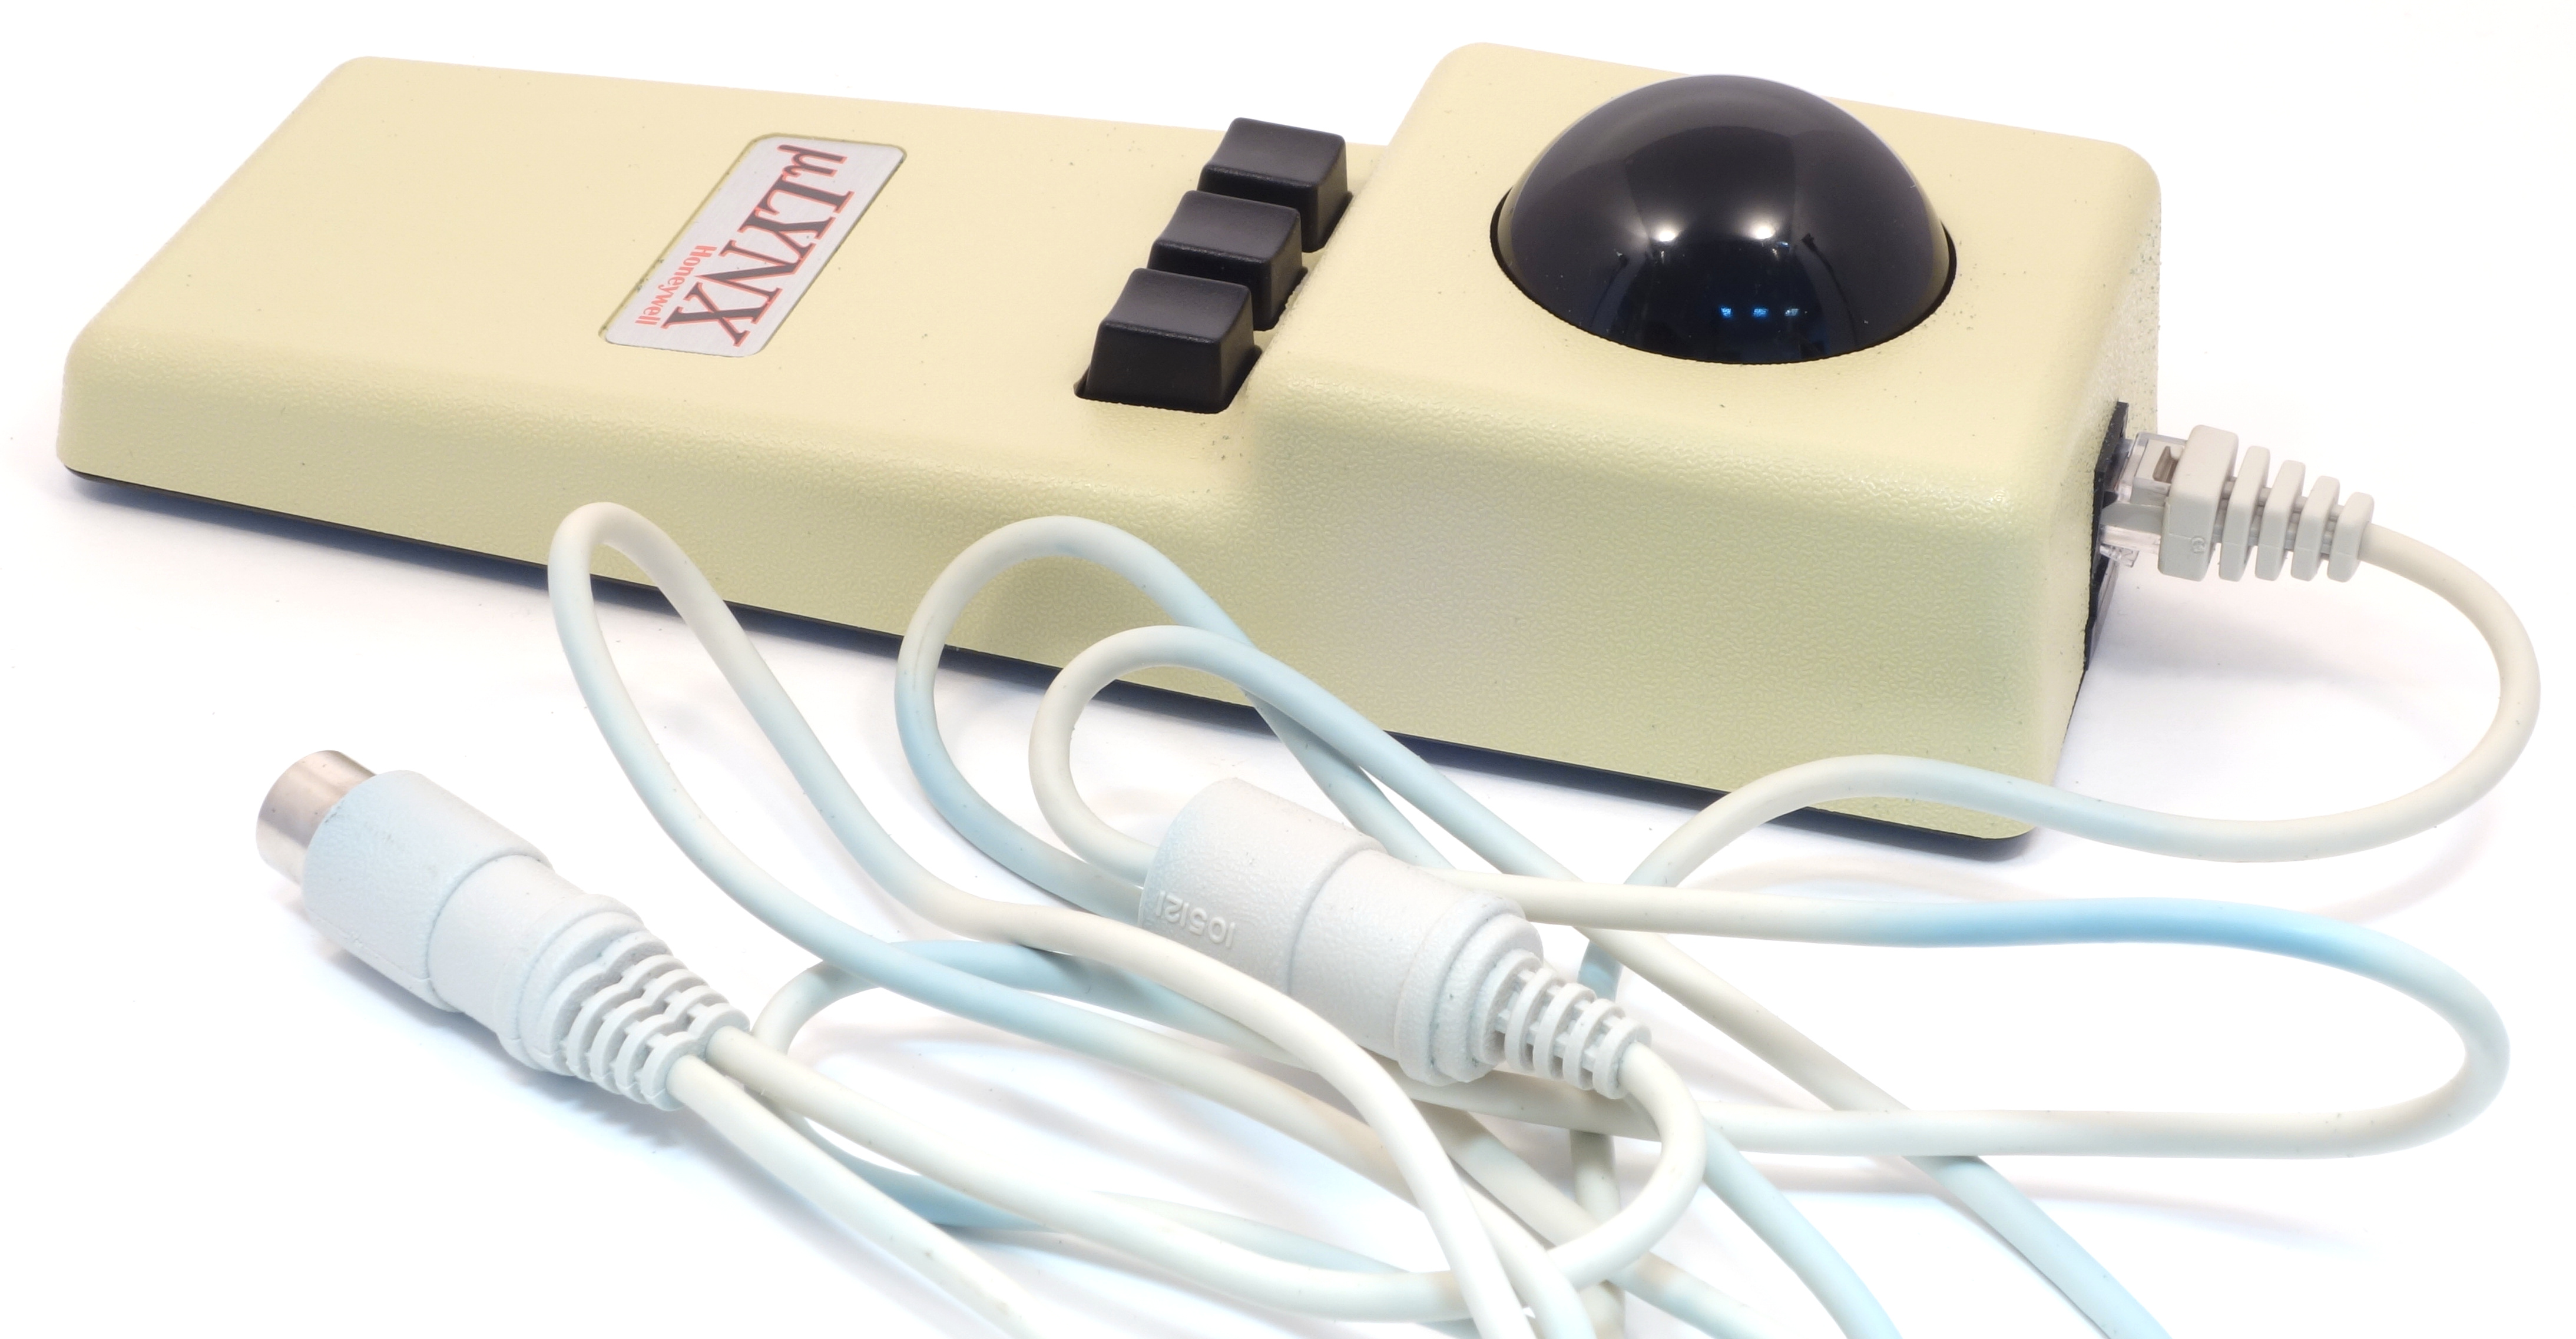
\includegraphics[scale=0.4]{1986_honeywell_microlynx_trackball/pic_60.jpg}
    \caption{Внешний вид трекбола microLYNX}
    \label{fig:microLYNXPic}
\end{figure}

Устройство оснащено большим черным шаром в бежевом корпусе с вытянутой подставкой
под запястье \ref{fig:microLYNXTopBottom}. Перед шаром расположены три кнопки по форме соответствующие классической полноразмерной клавиатуре. Шар плотно прилегает к краям отверстия в корпусе, что неплохо защищает от попадания мусора внутрь трекбола, но делает извлечение шара для чистки невозможным без разборки корпуса.

\begin{figure}[h]
    \centering
    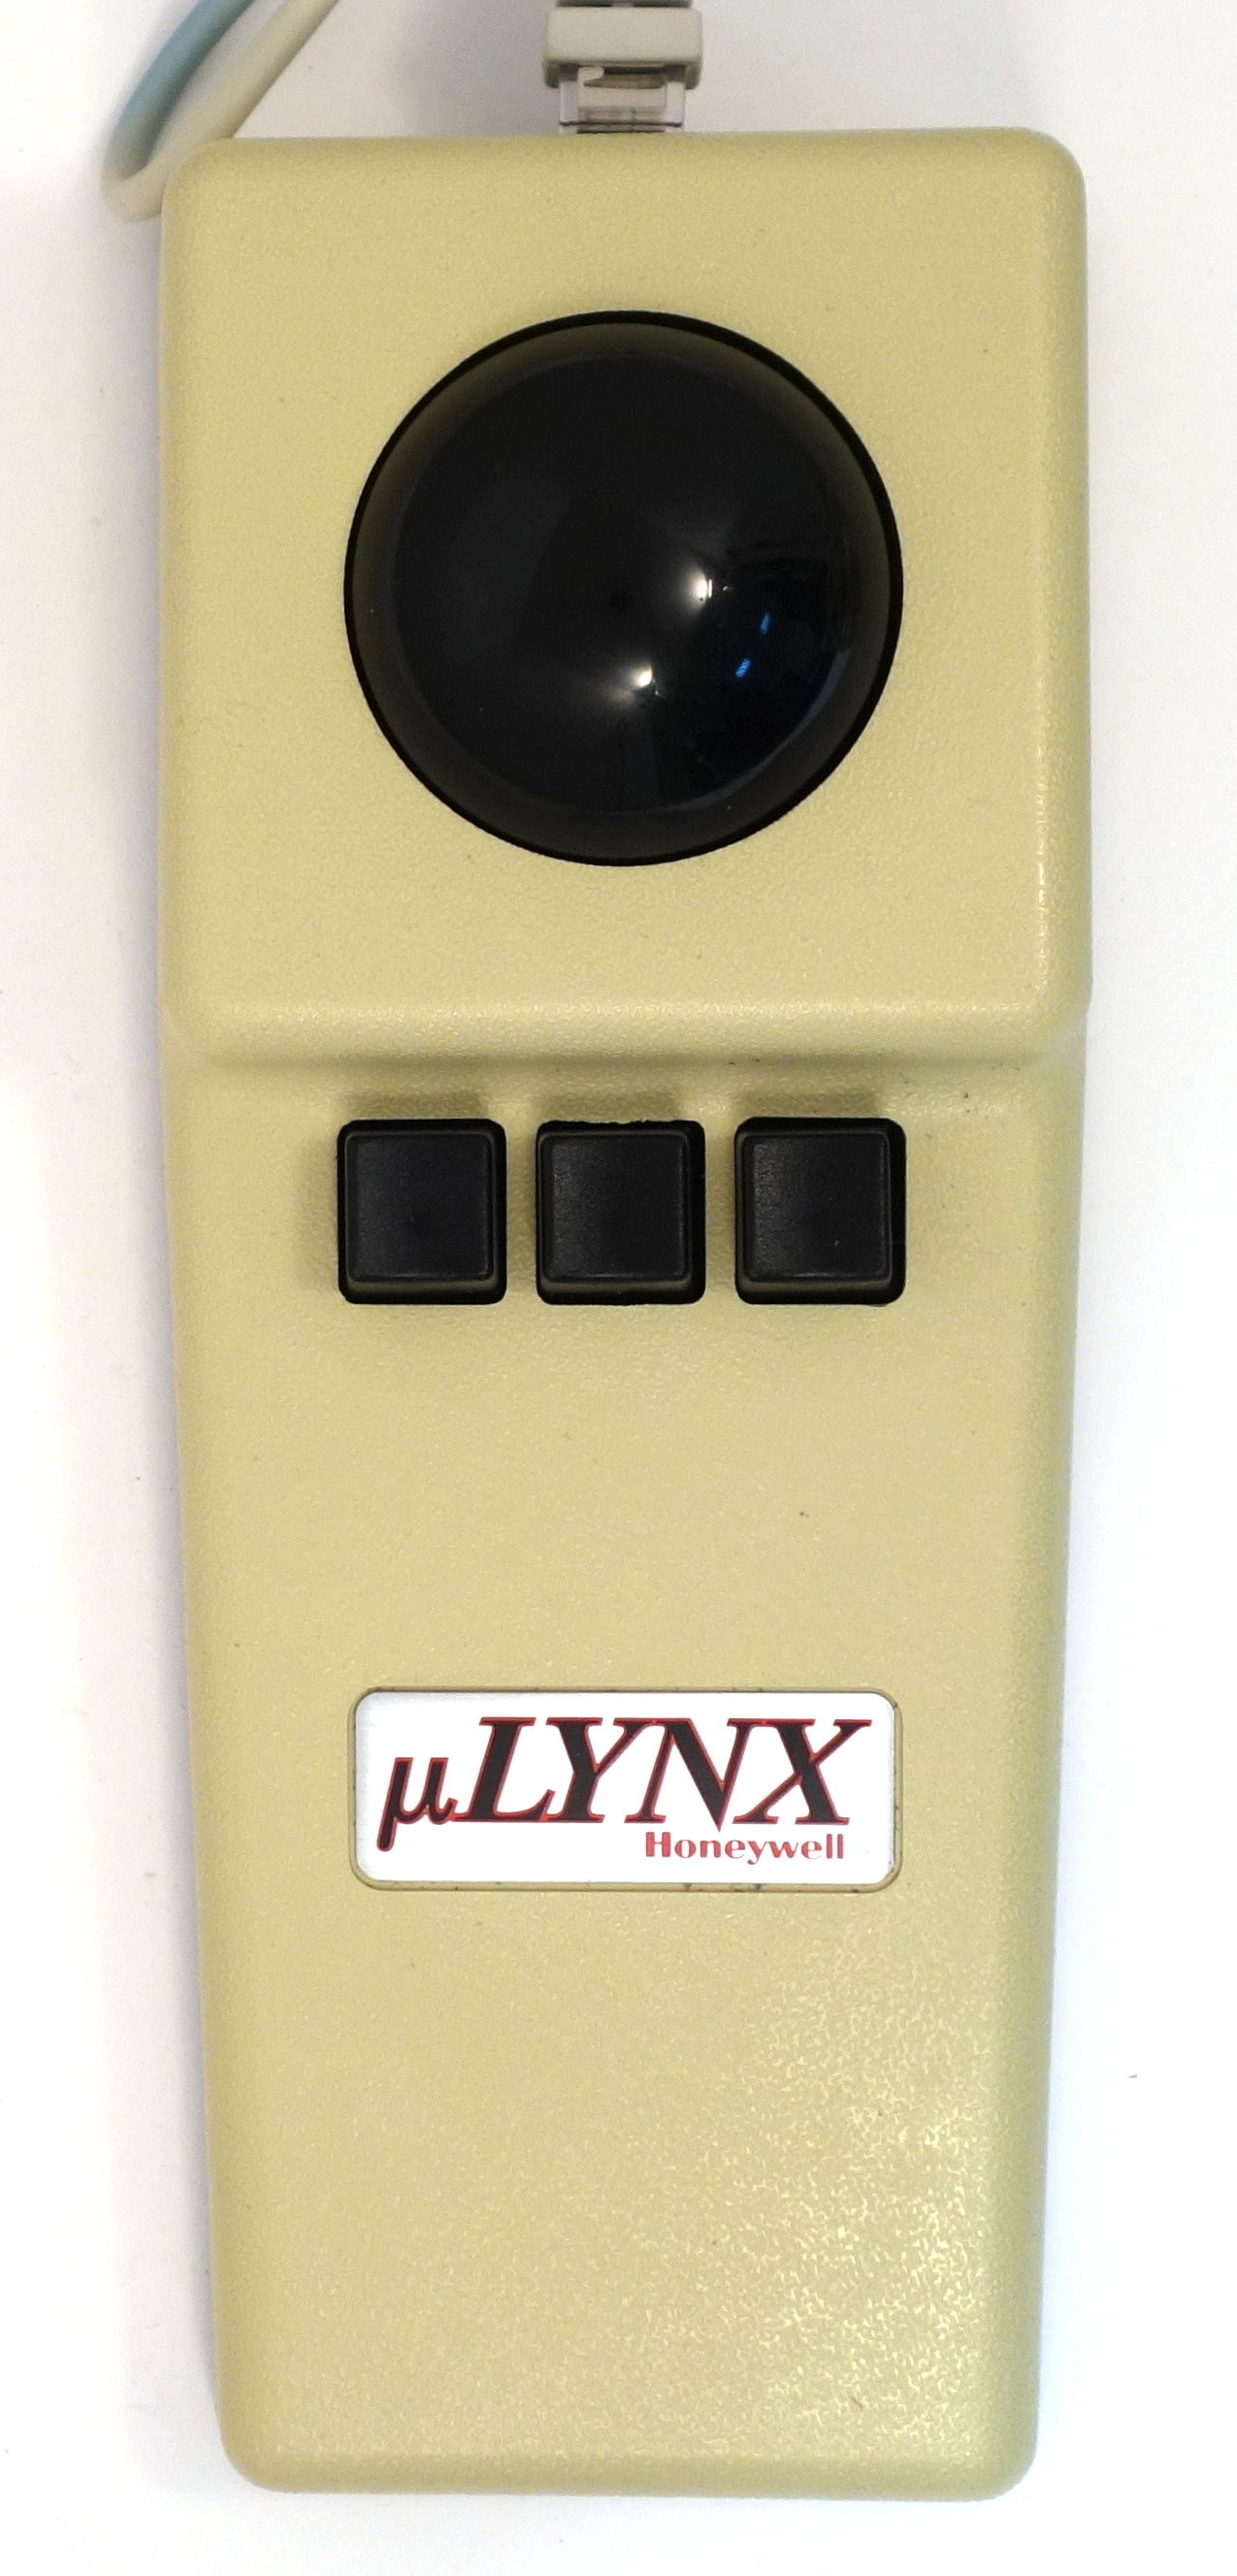
\includegraphics[scale=0.4]{1986_honeywell_microlynx_trackball/top_30.jpg}
    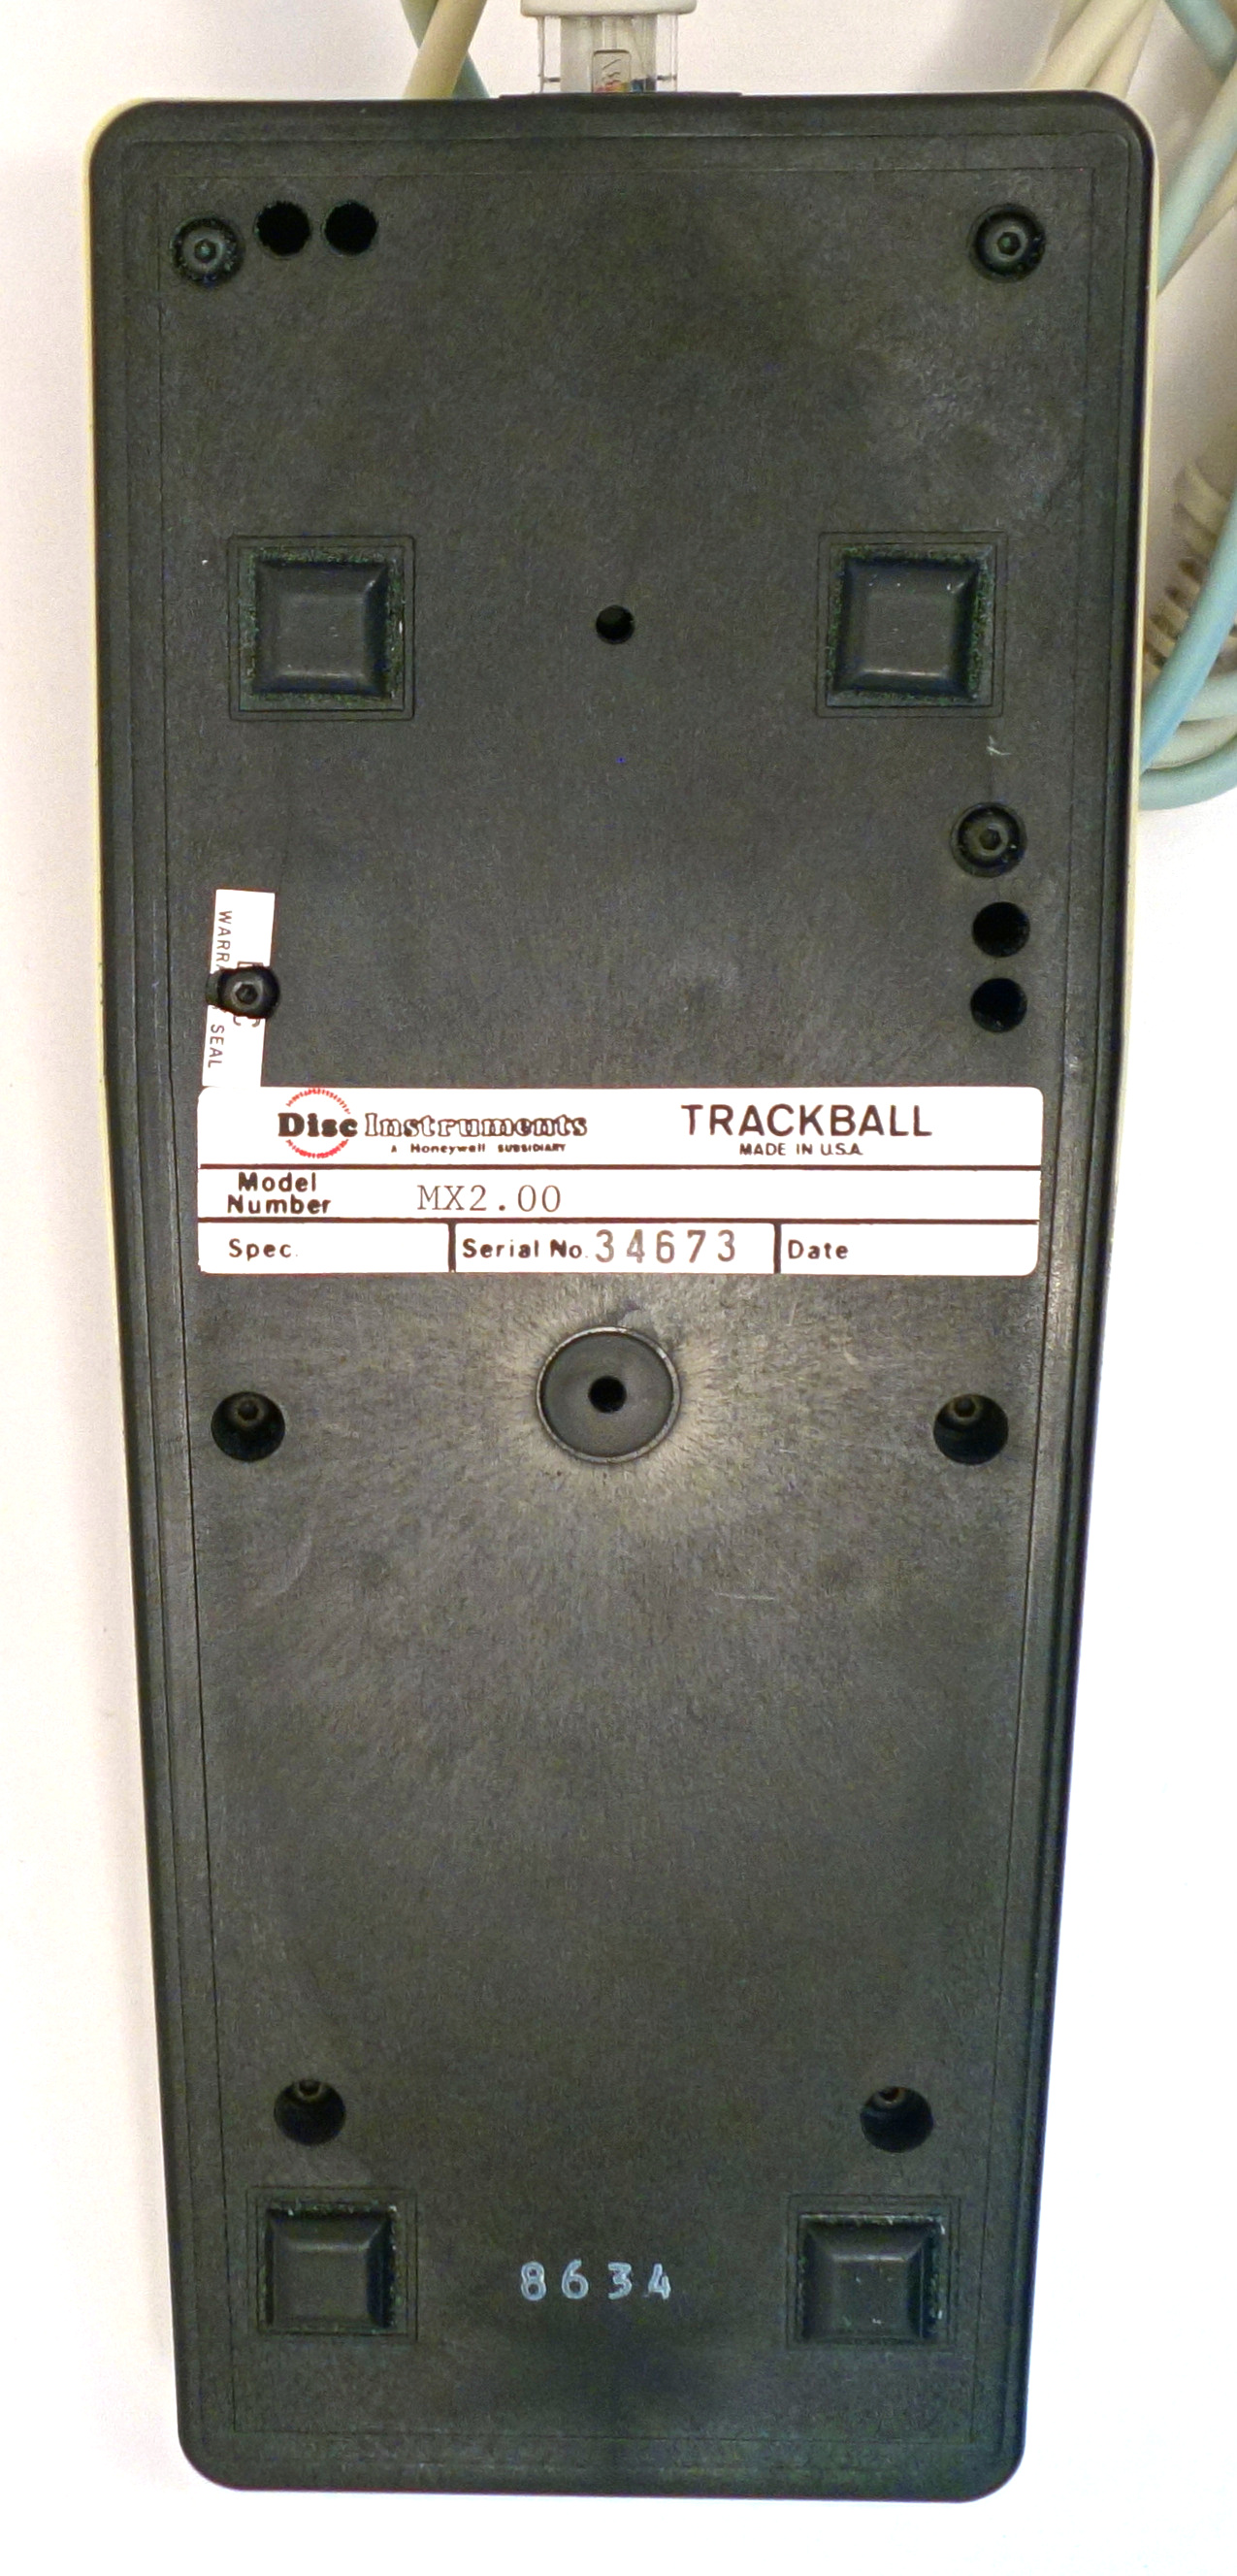
\includegraphics[scale=0.4]{1986_honeywell_microlynx_trackball/bottom_30.jpg}
    \caption{microLYNX, вид сверху и снизу}
    \label{fig:microLYNXTopBottom}
\end{figure}

Трекбол выпускался в нескольких модификациях, различающихся интерфейсом подключения. Модель comLYNX отличалась названием и тем, что подключалась к последовательному порту, а microLYNX использовал в качестве интерфейса подключения порт клавиатуры, фактически включаясь в разрыв клавиатурного кабеля.

При первом включении питания microLYNX переводится в <<текстовый режим>>, при котором поворот шара производит тот же эффект, что и нажатие клавиш курсора на клавиатуре: при движении шара трекбол генерирует и посылает в компьютер скан-коды курсорных клавиш. Кнопки трекбола
полностью программируются, и пользователь может настроить их на выдачу до 30 символов каждая в виде макросов. Также можно настроить
скорость перемещения курсора (частоту генерирования кодов курсорных клавиш) в текстовом режиме.

Для графических программ драйвер, которым комплектовался microLYNX, может эмулировать мышь Microsoft. В этом случае пользователь может использовать трекбол для перемещения курсора и перетаскивания при выделении текста или перемещении графического элемента. Для перетаскивания могут использоваться две внешние кнопки, расположенные перед шаром.

\begin{figure}[h]
    \centering
    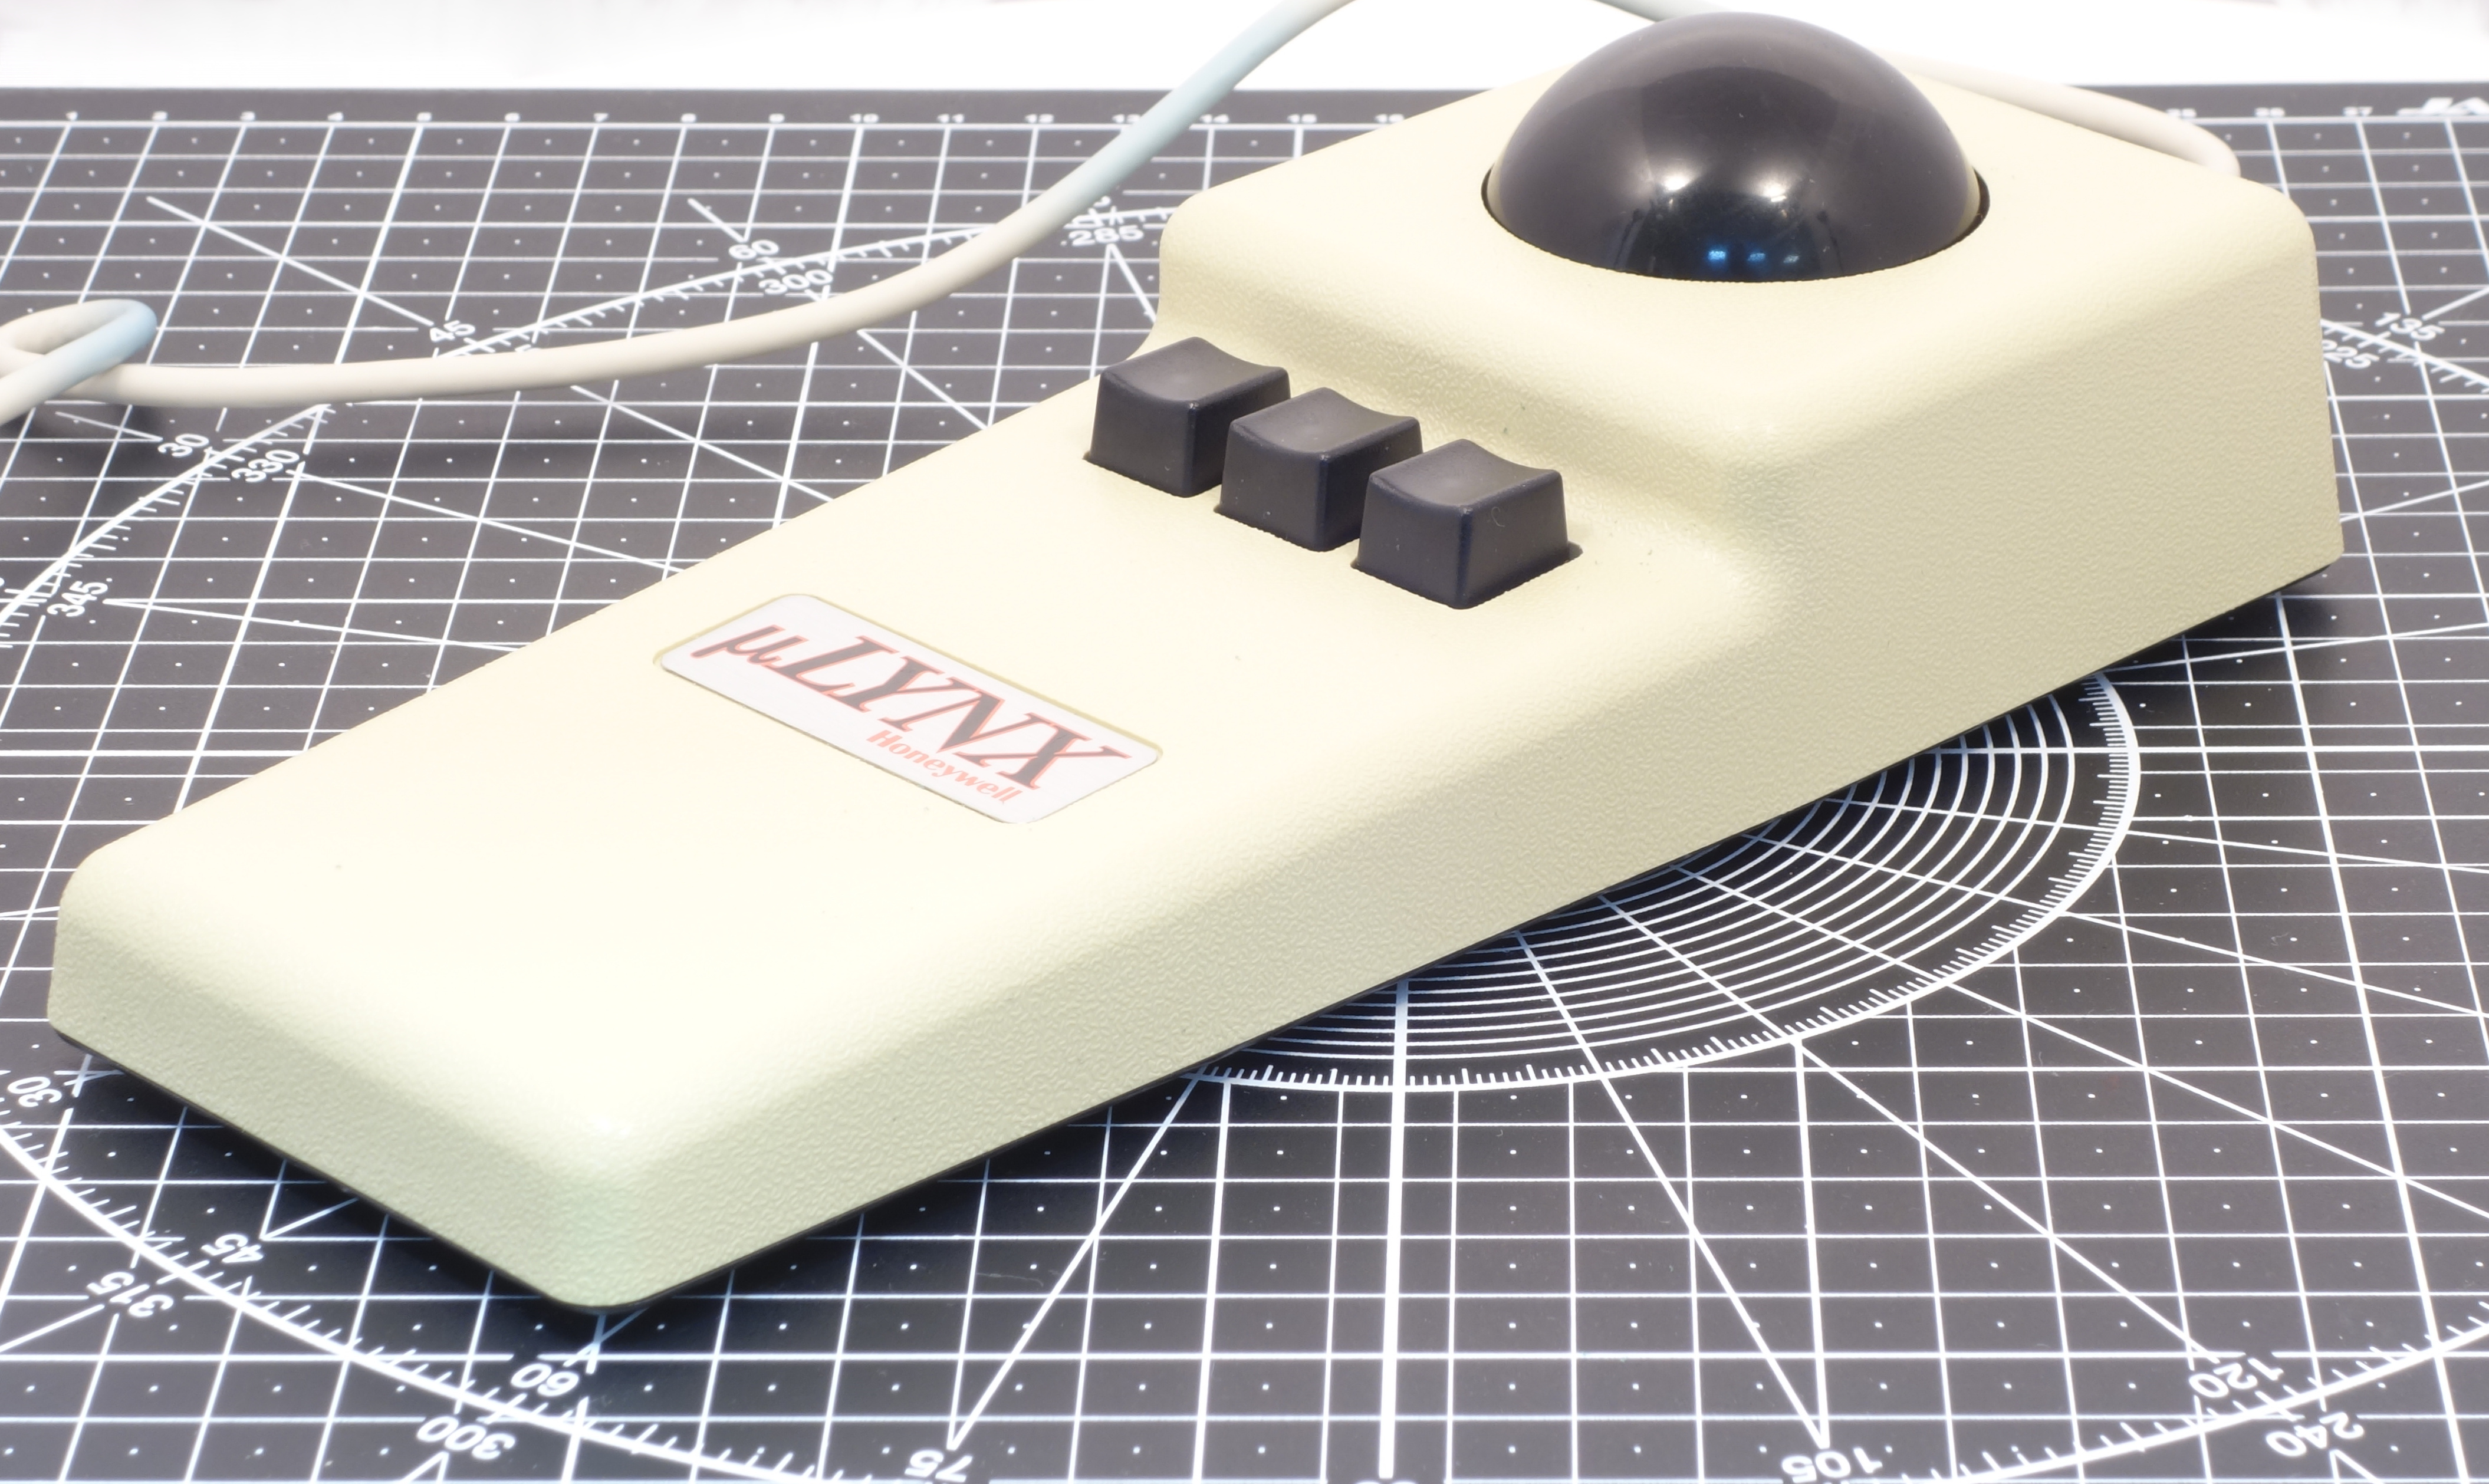
\includegraphics[scale=0.3]{1986_honeywell_microlynx_trackball/size.jpg}
    \caption{Трекбол microLYNX на размерном коврике с шагом сетки 1 см}
    \label{fig:microLYNXSize}
\end{figure}

Однако, учитывая размеры устройства (рис. \ref{fig:microLYNXSize}), удерживать нажатой кнопку, пока происходит
перемещение шара "--- это в лучшем случае сложный маневр. Honeywell решила
эту проблему на родственном данному трекболу устройстве comLYNX, используя
среднюю кнопку в качестве <<защелки>> перетаскивания. Сначала выполняется нажатие средней кнопки, затем левой либо правой, и это
программно фиксирует выбранную кнопку в нажатом положении. Нажатие любой из трех кнопок повторно
отключает данный режим. Однако в microLYNX эта функция не поддерживается.

Оба трекбола поставляются с двумя наборами программ: драйвером для DOS, эмулирующим мышь Microsoft, и отдельной резидентной программой для DOS, которая показывает всплывающее меню, а также позволяет запрограммировать клавиатурные макросы для кнопок трекбола и перемещения курсора.

\begin{figure}[h]
    \centering
    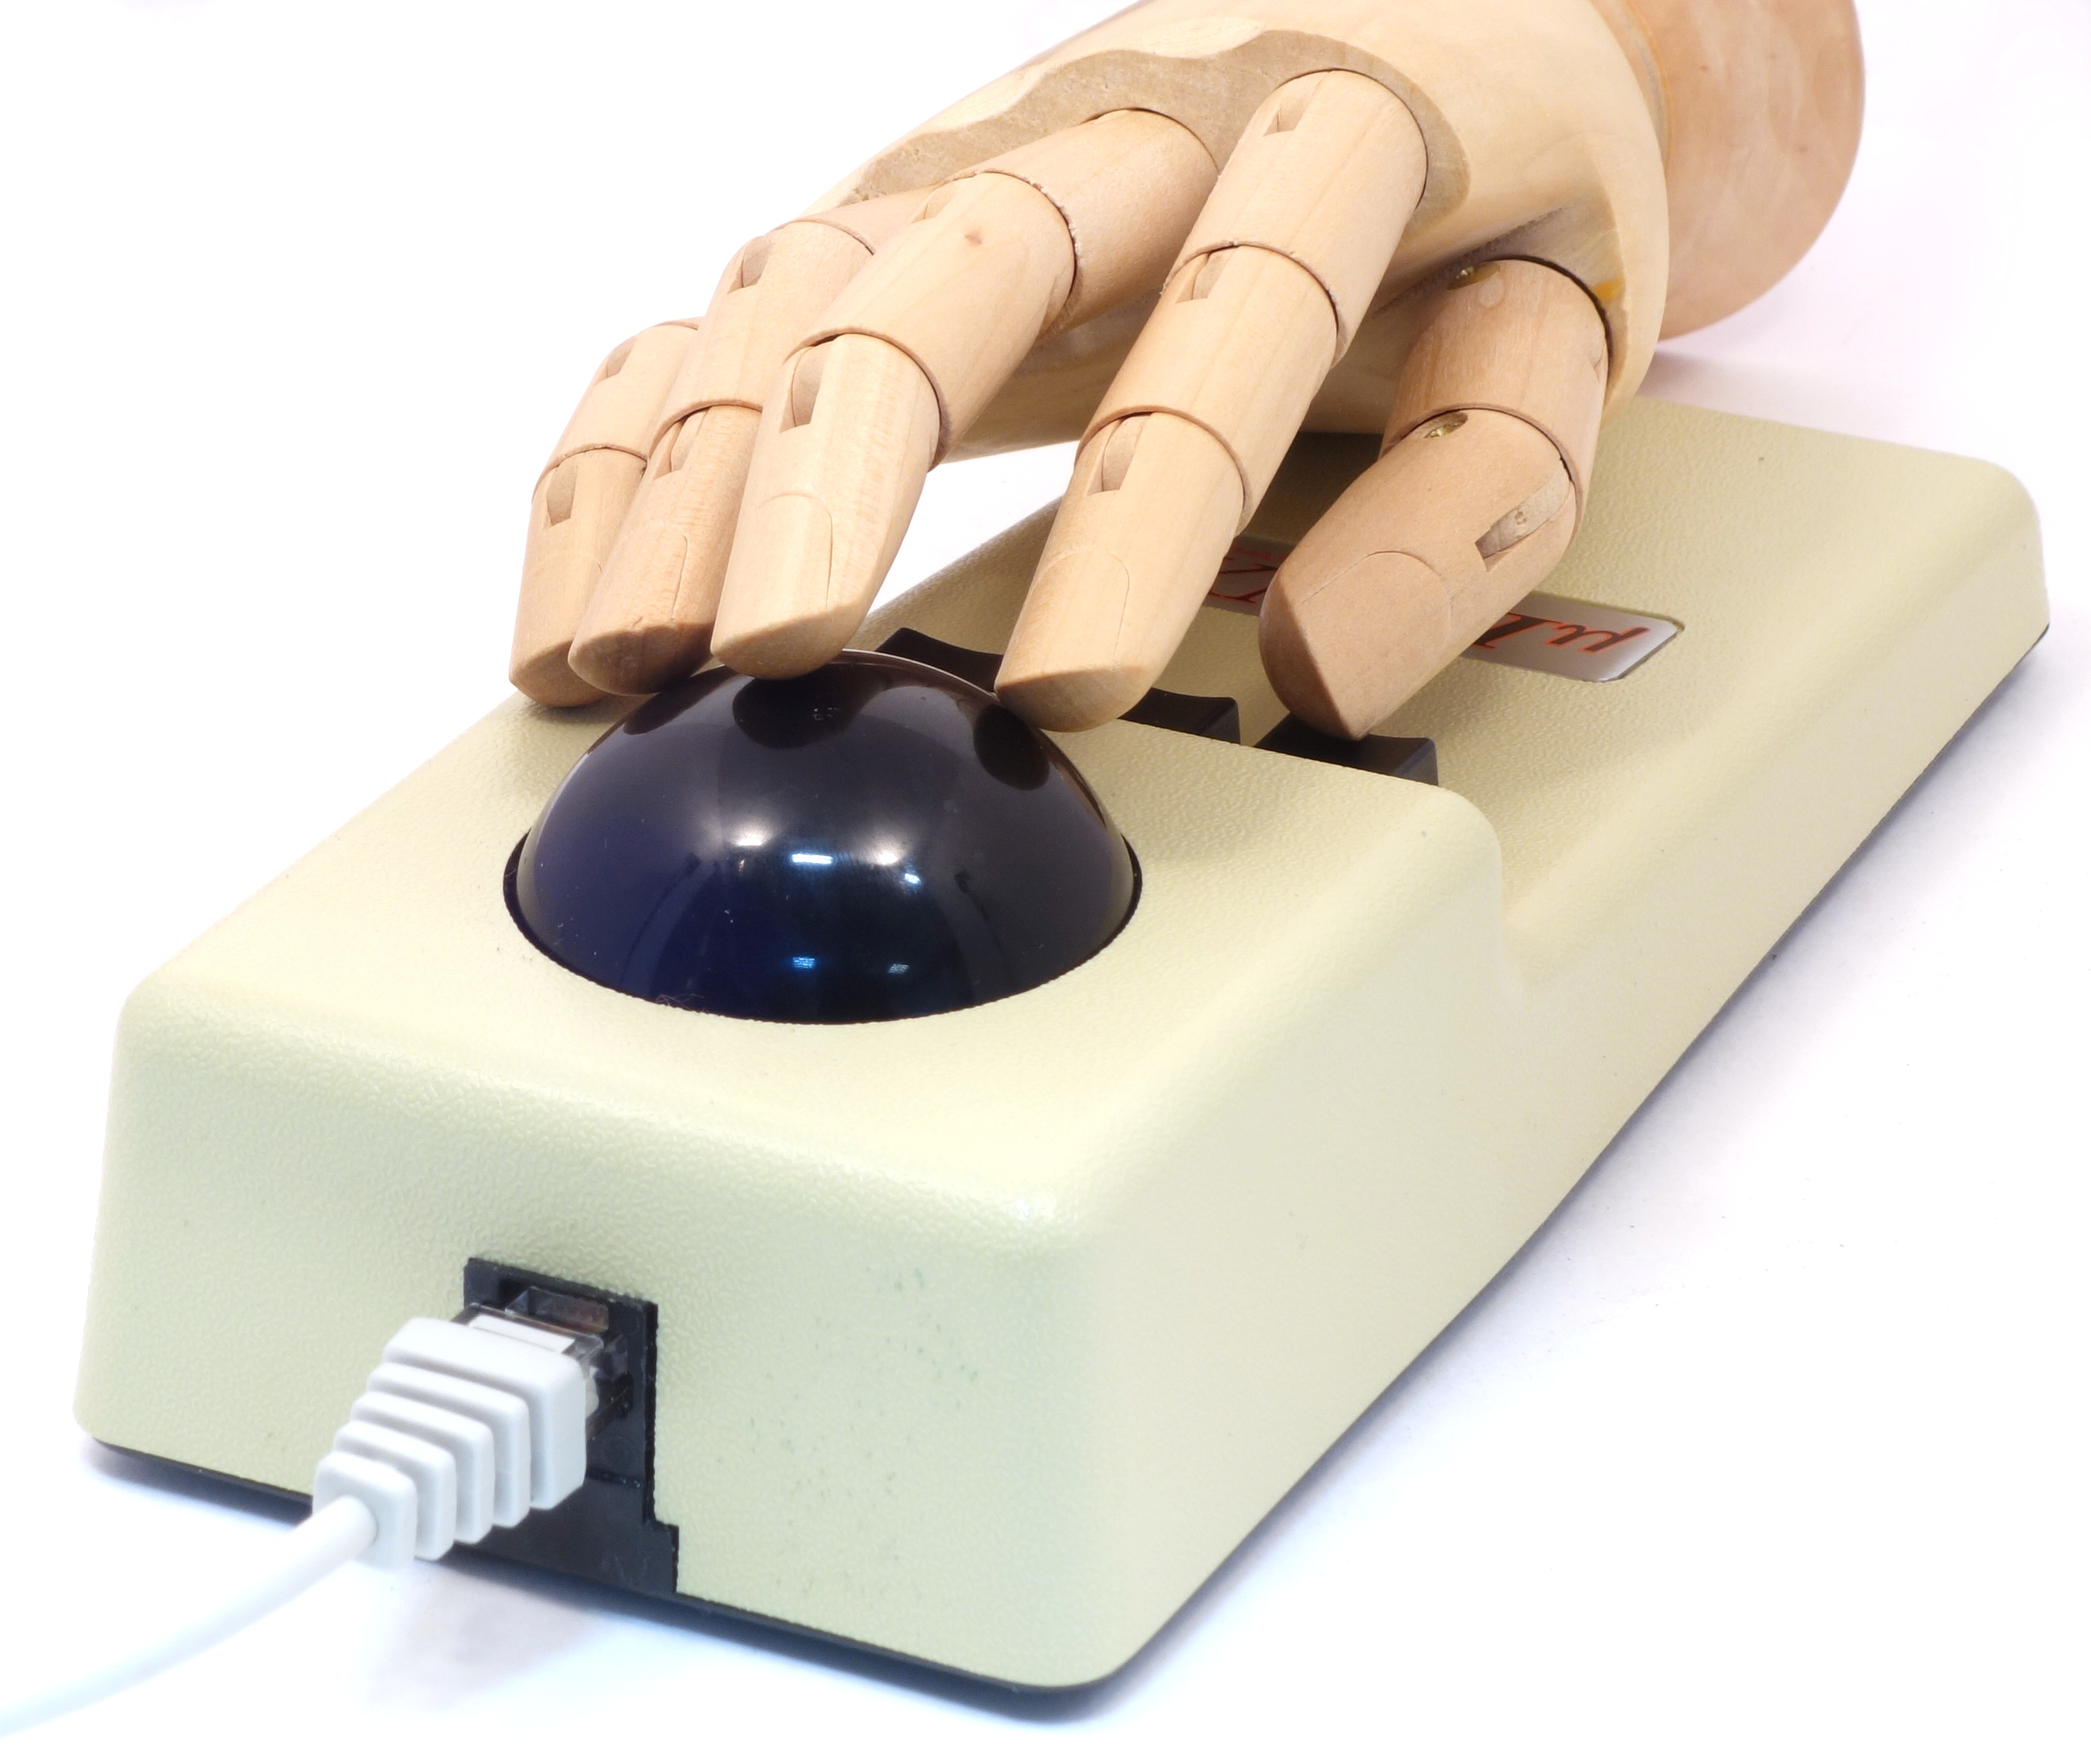
\includegraphics[scale=0.4]{1986_honeywell_microlynx_trackball/hand_60.jpg}
    \caption{Трекбол microLYNX в комплекте с моделью руки человека}
    \label{fig:microLYNXHand}
\end{figure}

В отношении эргономики размеры трекбола, подставка под запястье, а также скругленные грани и углы создают достаточно комфортные условия для работы. Однако кнопки расположены достаточно далеко от шара, и существенно ниже по высоте, что лишает пользователя как возможности нажимать их одной рукой без перемещения кисти, так и двумя руками, поскольку при вращении шара кнопки закрыты ладонью (рис. \ref{fig:microLYNXHand}). Поэтому microLYNX трудно использовать в условиях, требующих интенсивной работы с постоянным чередованием перемещений курсора и нажатием кнопок.

\begin{figure}[h]
    \centering
    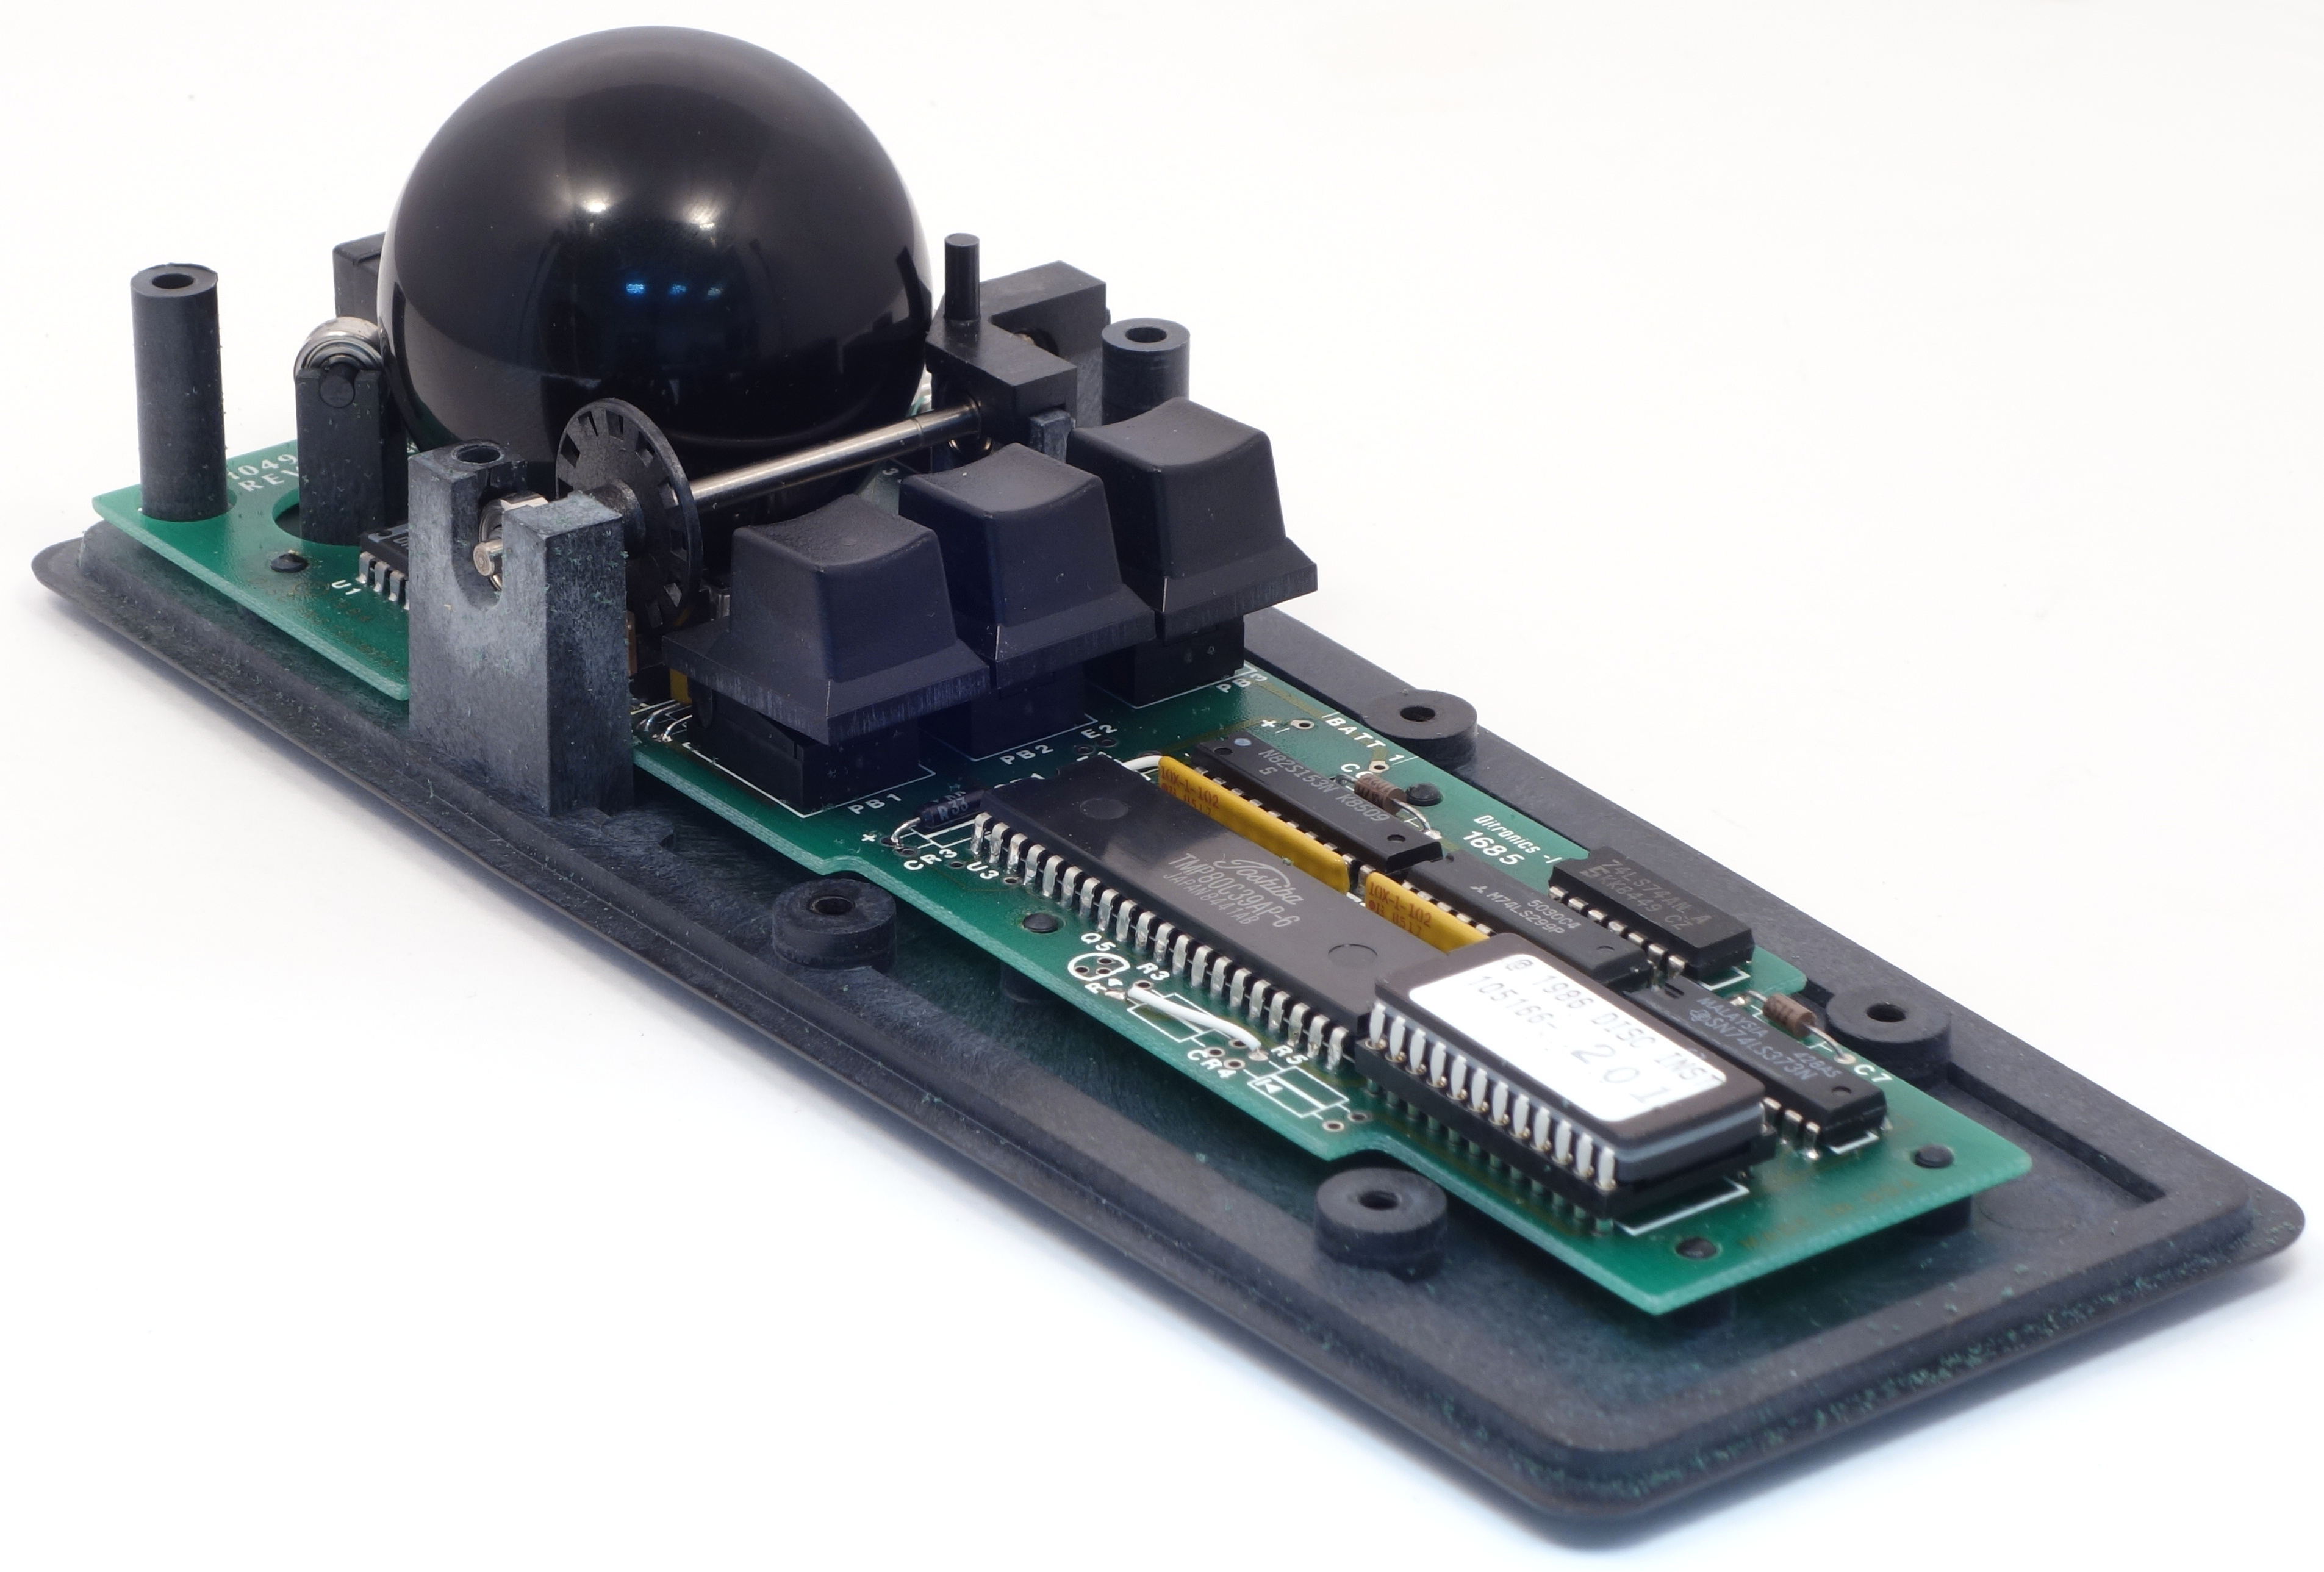
\includegraphics[scale=0.5]{1986_honeywell_microlynx_trackball/inside_60.jpg}
    \caption{microLYNX в разобранном виде}
    \label{fig:microLYNXInside}
\end{figure}

Внутреннее устройство данного трекбола показано на рис. \ref{fig:microLYNXInside}, что позволяет классифицировать его как оптомеханическое устройство. Также следует отметить, что ролики реализованы с использованием подшипников и валов из нержавеющей стали, что обеспечивает максимальную надежность и долговечность конструкции. Высокая надежность трекбола и эргономика, хорошо подходящая для ряда технических задач, сделали данную модель <<долгожителем>>: устройство не меньше десяти лет выпускалось для индустриальных применений под различными марками, полностью сохранив внешний вид и механическую часть конструкции.
 
\begin{thebibliography}{9}
\bibitem {mouses} Trackballs: Stationary mice // PC Magazine. August 1987, page 199-202
\end{thebibliography}
\end{document}
